\question 若一棵二叉树的前序遍历序列为a,e,b,d,c,后序遍历序列为b,c,d,e,a,则根结点的孩子结点(
)
\par\twoch{\textcolor{red}{只有e}}{有e、b}{有e、c}{无法确定}
\begin{solution}根节点一定是a,就有3种可能: ①a有左孩子,无右孩子。
②a无左孩子,有右孩子。 ③a有左孩子,有右孩子。
假设情况一成立,e,b,d,c即为左子树的先序序列,b,c,d,e即为左子树的后序序列,明显e为左子树的根节点,且左右孩子皆有(考虑单个子树的话,先序bdc与后序bcd矛盾)。故该左子树可能如下图所示。
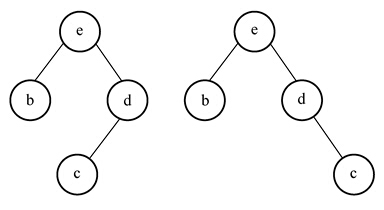
\includegraphics[width=4.00000in,height=2.18750in]{computerassets/8477d425f479b1f532486ea3861e03b0.jpeg}
假设情况二成立,得出e为右子树的根节点,右子树的可能情况也同上。
假设情况三成立,e即为左子树,b、d、c即为右子树的先序序列,b、c、d即为右子树的后序序列,该先序序列与后序序列矛盾。
所以该二叉树只有一个孩子结点e。 【总结】
由二叉树的中序序列和后序序列、中序序列和先序序列、中序序列和层次序列都可以唯一确定一棵二叉树。但不能由先序序列和后序序列唯一确定一棵二叉树。
任意两个先序序列和后序序列,不能唯一确定一棵二叉树,如本题的情况。同时,也可能没有一棵二叉树符合这两种遍历序列。如先序ab,后序ab即无二叉树与之对应。
\end{solution}
\question (重庆大学,2004年)一棵二叉树节点的( )可唯一确定一棵二叉树
\par\twoch{\textcolor{red}{前序序列和中序序列}}{前序序列和后续序列}{中序序列}{后序序列}
\begin{solution}能唯一确定原二叉树的遍历方式组合是:前序+中序,或者是后序+中序,而前序+后序不能确定唯一的二叉树
\end{solution}
